\chapter{Introduction}

\section{Overview}

What is Backend as a Service ? It is a way for developers to link their applications to backend cloud-based storage and services.Back-end as a service or BaaS is best described by a tech analyst who refers to it as "turn-on infrastructure" for mobile and web apps. Basically it's a cloud computing category that's comprised of companies that make it easier for developers to setup, use and operate a cloud backend for their mobile, tablet and web apps \cite{kinveywebsite}.  

\section{Project Objectives}
The aim of the this project is to develop a template for the development of mobile applications. This template is to help improve the development of modern mobile applications for new and experienced developers. This is achieved by providing services to help with the different phases of development. The project aim is to create a complete package that will enable new and experience developers speed up in the following areas:

\begin{enumerate}
  \item Development
  \item Testing 
  \item Production
\end{enumerate}

The project deliverables to aid with the three phases include the following:

\begin{enumerate}
  \item Dashboard
  
    The dashboard is a control panel that simplifies configuring applications. It also has data visualization to help improve the user experience when using the applications.
  \item Mobile Back-end as a Service
  
    This is a model for developers to link their applications to the backend cloud storage and application programming interfaces (API's) exposed to provide the communication with the list of services above.
  \item iOS Framework
  
    The services above need a way to communicate from back-end to the mobile apps. This is accomplish by providing a custom software development kits (SDKs).
\end{enumerate}

\section{Project Overview}

\begin{figure}[h]
    \caption{Project Overview 2}
    \centering
    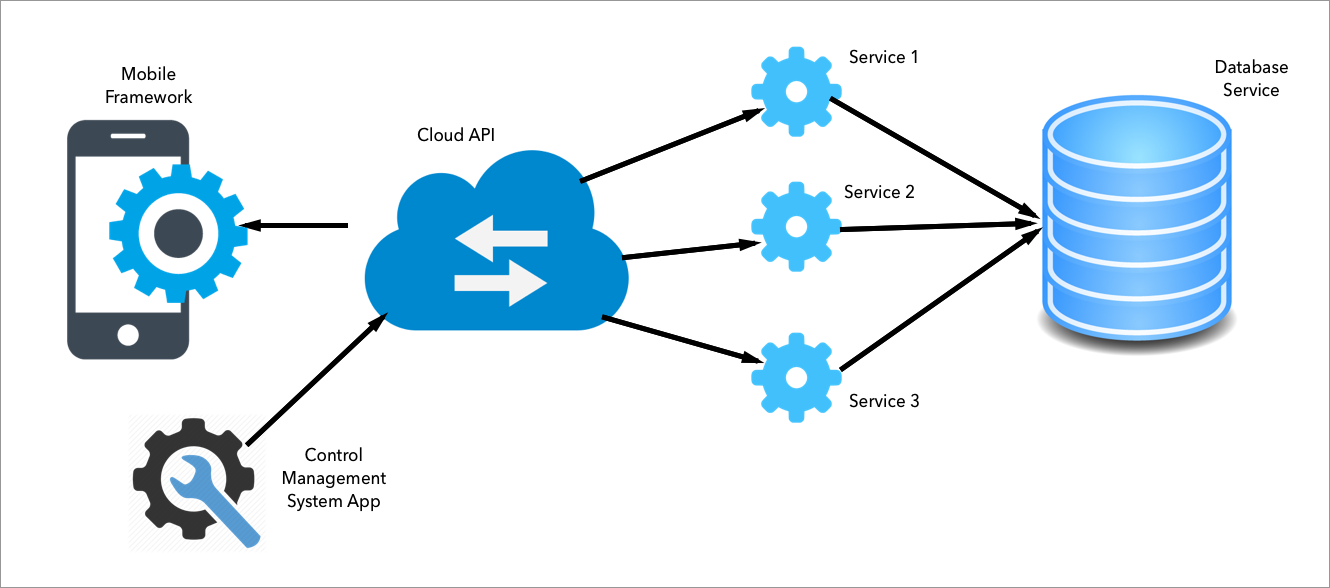
\includegraphics[width=100mm]{images/overview}
    \label{fig:project_overview1}
\end{figure}

\begin{figure}[h]
    \caption{Project Overview 2}
    \centering
    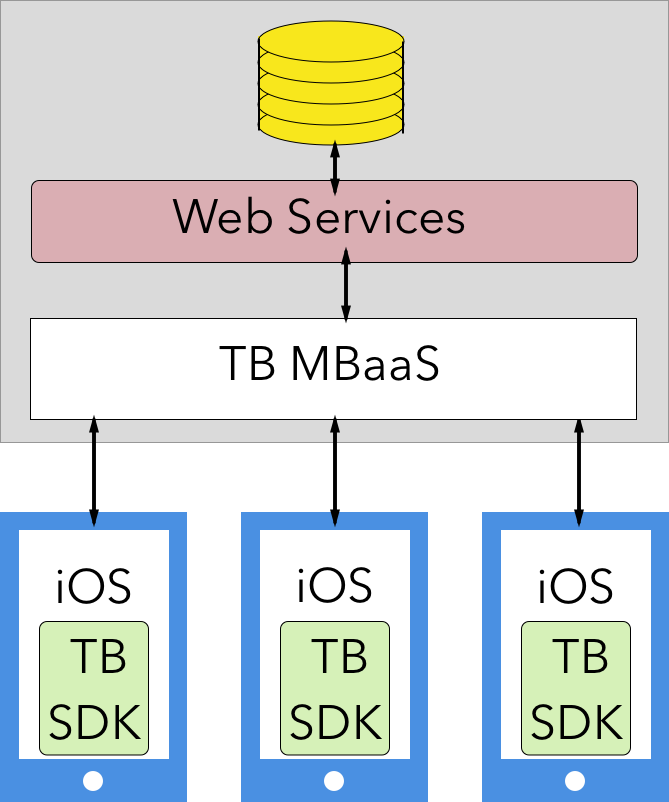
\includegraphics[width=60mm]{images/app_overview}
    \label{fig:project_overview2}
\end{figure}


\section{Project Challenges}

The key challenge of the project was to find what developers functional requirements looking for when choosing a mobile backend as a service what current providers do not offer. This required setting up meetings with professional mobile developers and get their opinion on the project.

The big challenge faced was to find a way to enhance the developing stage of any application, giving more power to the developer when the application has been published. This lead to another challenge to see how far Apple would allow applications to be configured after published.

\section{Chapter Walk-through}

\paragraph{Chapter 2 Research}

This chapters discusses the alternative existing solutions to the problem. It also goes into the potential technologies that could be used in the project along with the resultant findings. The technologies discussed will be what web server to use, the programming language and what the dashboard be development in. This chapter will include surveys and out-sourced discussions with professional mobile developers.

\paragraph{Chapter 5 Architecture}

The architecture chapter will show the overview diagram of the complete project, along with diagrams of the individual services.

\paragraph{Chapter 4 Design}

This chapters goes into the design of the projects. What methodologies will be used?, and go into detail of the list of features already mentioned in project objectives section.

\paragraph{Chapter 5 Development}

This chapter will discuses the different deliverable in the project in order to achieve the project aim. It will contain detail description of the features that will be used to aid in mobile application development.

\paragraph{Chapter 6 Implementation}

Implementation chapters explains how to use different deliverables included in the project. Along with code snippets which show how to set up the system and use the SDK.

\paragraph{Chapter 7 Testing/Evaluation}

This chapter will give an overview of all testing carried out including test-driven approach and unit service testing. The evaluation section discusses the review given from the out-source professional developers. The review not only includes their feedback using the system but also their recommendations where to from here. 

\paragraph{Chapter 8 Conclusion}
The conclusion chapter contains a summary of the project overall and ends with a reflection of the project.

\paragraph{Chapter 9 Cases}
The conclusion chapter discusses the meetings and evaluations with out-sourced professional mobile app developers.